%!TEX root = ../template.tex
%%%%%%%%%%%%%%%%%%%%%%%%%%%%%%%%%%%%%%%%%%%%%%%%%%%%%%%%%%%%%%%%%%%%
%% chapter4.tex
%% NOVA thesis document file
%%
%% Chapter with lots of dummy text
%%%%%%%%%%%%%%%%%%%%%%%%%%%%%%%%%%%%%%%%%%%%%%%%%%%%%%%%%%%%%%%%%%%%
\chapter{Approach and Planning}
\label{cha:approach_and_planning}

Since two members of the FCT-UNL institution are part of the FitoAgro project and dissertation topics shall not overlap, the server processing of this data is not mentioned in this work. Data collection is, ultimately, a server routine but also an important part of the work described in this very document. This being said, this work is being closely integrated to the work in \emph{André Malafaia}'s dissertation and the technological stack is going to be decided by both during the first days of dissertation work.

The pest monitoring protocol is going to be closely followed \textit{in situ} to sucessfully iterate the proposed framework as in an agile methodology: small development cycles should be made on the framework/applications and testing on the field as features are released. The interface will be tested directly with the users in a task-based test so see if the user is able to perform the directed task or not. 

\section{Third-Party Data Collection}

The work proposed in this document starts by collecting data from weather and soil stations. Integration with FitoAgro stations (WiseCrop \cite{wisecrop} and TerraPro \cite{terrapro}) will provide field variables. This means that, against the precision agriculture methodology refered in \ref{sec:precision_agriculture}, it will be assumed that the measurements made by a single point in the field are constant throughout the entire field (for weather and soil sensors). If some farming fields have no nearby weather stations, the possibility of combining free satellite data (low temporal and geospatial resolution) is going to be analysed.

The figure \ref{fig:vis_pers_lowlevel} shows an example of a farming field visualization with low level of detail: big areas have the same variables due to low density of sensorial devices, in most cases only 1 sensor of a type per farming field). 

\begin{figure}[htbp]
  \centering
  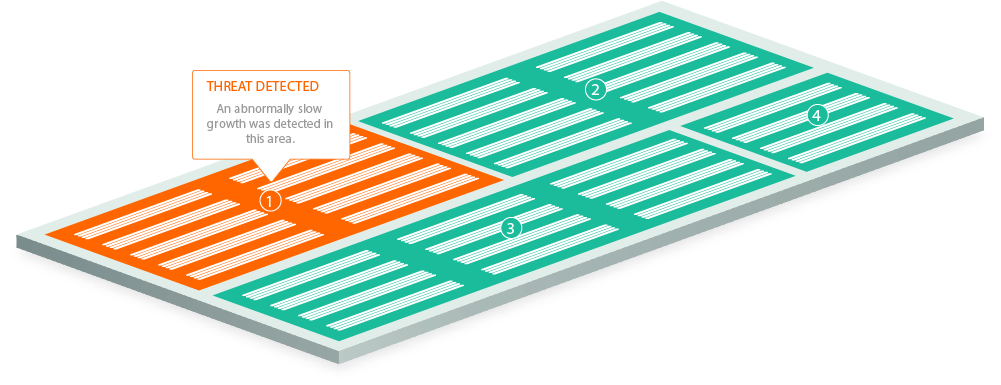
\includegraphics[width=0.8\linewidth]{vis_pers_lowlevel}
  \caption{Visualization of a farming field with a second level of detail: Plot. This assumes that 4 sensors of each type are available in the farming field represented, one for each plot.}
  \label{fig:vis_pers_lowlevel}
\end{figure}

The FitoAgro project is planned to be 4 years long. If during the first year (the time of development of the dissertation) the pest monitoring system of the FitoAgro project evolves in requisites (more spatial resolution is needed), efforts to gather more information will be made. This can mean paid satellite services (\textit{WorldView-3}) for more resolution on intra-field data collection or soil sensor meshes collecting ground information as of described in \ref{sec:soil_station}. Satellite data would mean getting crop growth levels, nutrients, soil moisture without having to install any sensors, but paying a fixed fee per hectare. Since every sensorial device has a cost, economic viability of new data sources will be fully studied.

\section{Tree-level maps for precision agriculture}

The only data that is to be collected at tree-level (measurements by tree), on this first stage of the project, are pest biological observations. Examples of tree-level visualizations for the FitoAgro project being developed can be analysed in figures \ref{fig:vis_pers_highlevel} and \ref{fig:vis_2d_highlevel}. These present the very first prototypes of the user interface design on how data is to be communicated in a user-friendly way. These are still work in progress so will, most likely, change during the course of this dissertation work.

\begin{figure}[htbp]
  \centering
  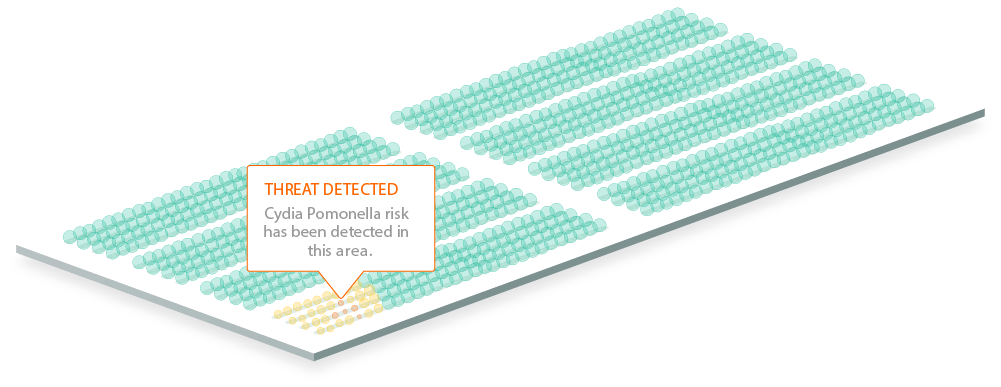
\includegraphics[width=1\linewidth]{vis_pers_highlevel}
  \caption{3D Visualization work for the FitoAgro project under development.}
  \label{fig:vis_pers_highlevel}
\end{figure}


\begin{figure}[htbp]
  \centering
  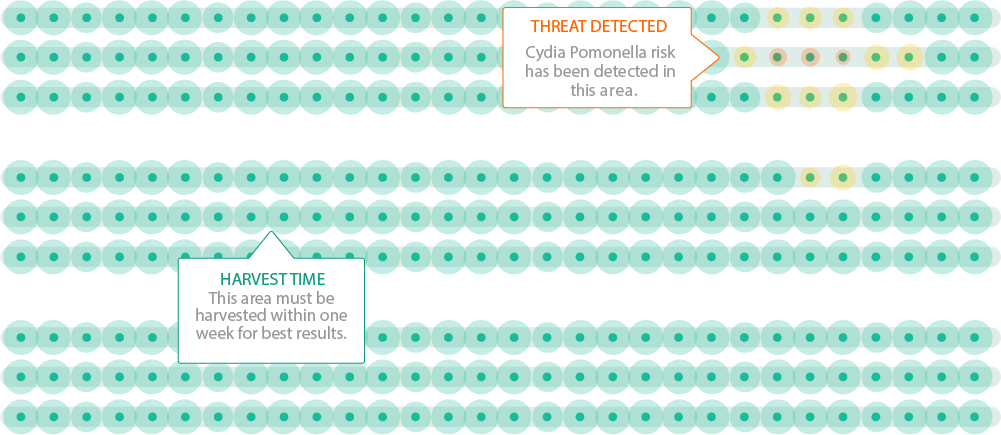
\includegraphics[width=0.7\linewidth]{vis_2d_highlevel}
  \caption{2D Visualization work for the FitoAgro project under development.}
  \label{fig:vis_2d_highlevel}
\end{figure}

These, even if prototypes, present a good starting point for both the mobile and web interfaces (assuming 2D for smaller devices and 3D for laptop/desktop, this premise will be tested with users). 

As refered in section \ref{sec:mobile_web_app}, mobile and laptop/desktop provide different interaction patterns for the user. Two very different use cases were presented and, for the analysis of the field variables, bigger screens fit more information and information with more details. This being said, the creation of a web application to support user analysis of the farming variables is of importance to ease-out the visualization process and for convenience.

\section{Web Application}

As refered in section \ref{sec:mobile_web_app}, mobile and laptop/desktop provide different interaction patterns for the user. Two very different use cases were presented and, for the analysis of the field variables, bigger screens fit more information as well as information with more details. This being said, the creation of a web application to support user analysis of the farming variables is of high importance to ease-out the visualization process and for convenience since most of the analysis work is not performed in the farming field but in the office.

The web application should present visualizations of the field on a temporal manner, attribute based maps such as risk, weather, soil temperature, wind direction, phenological stage, pest observations etc. using 2D/3D layouts depending the user preference. It shall incorporate several fields and one or more plots per field. Each plot will have data from weather, soil and biological observations as major events in the production cycle: pesticide use dates, phenological stages of the crop, water leaks etc. Like the figure \ref{vis_pers_highlevel} suggests, variables will be mapped to color, size and possible form to aggregate several data sources in the same visualization.

The end-user will play a key-role in the development of these maps since only biologists and farming professionals know the details of what is important to track and what is not. It is planned to validate these maps with partner entities of the FitoAgro project as ISA (Instituto Superior de Agronomia). As biology experts, their insight on pest life cycle tracking is important to actually draw conclusions from the data being collected. 

\section{Enemy Monitoring Mobile Application}

On enemy monitoring, an event registering interface is going to be developed to be used directly in the field when registering biological observations. When biological measurements are being performed, geolocation of the device should be taken into account to sucessfully map the measurement taken to a specific point in the field (therefore, tree being monitored).

An example of the spreadsheet currently in use by the FitoAgro project managers and farmers can be found in \ref{fig:spreadsheet} and the problems with this method are described in \ref{subsec:spreadsheets}. The plan is to design, implement and test a mobile interface for data insertion directly from the tree being monitored and collect the attached geolocation from the client mobile device.

Measurements registered from the application will have capture counts of the tracked species, in-tree location (for enemy control protocols that register several measurements from each tree - pest life cycle analysis) as shown in figure \ref{fig:spreadsheet} and their geolocation. Some server side clustering techniques will be applied to ease out collection method since the tree id is not relevant but the geolocation of that tree. As show in figure \ref{fig:k-means}, K-Means or a similar clustering algorithm can be used to reduce GPS and user positioning errors. This is the normal use case: monitored trees are decided in the season opening and stay fixed during the whole production phase. Therefore, the number of trees being tracked is always the same, and so is their position. Variance in the location of the locations registered is to be discarded.

Due to the remote location of the farming fields, internet coverage may be scarse or even inexistent. The application should support no connection to the internet by storing all the measurements in local storage and later dispatching to the server when a connection is detected. This mechanism, often described as "Offline mode", is a common pattern in recent applications and shall be incorporated in the app to be developed. Alerts in the form of push-notifications, scheduling of events and monitored tree adjustment are optional, yet planned, features. These should be available in both client applications (mobile and web).

\begin{figure}[htbp]
  \centering
  \subcaptionbox{GPS locations from measurements \label{fig:k-means_black}}%
    {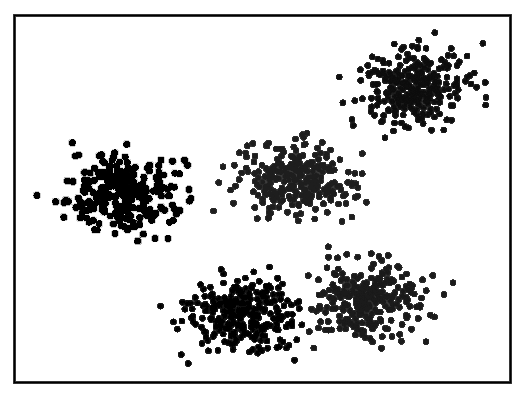
\includegraphics[width=0.5\linewidth]{k-means_black}}%
  \hfill  
  \subcaptionbox{Clustering applied to detect monitored tree locations \label{fig:k-means}}%
    {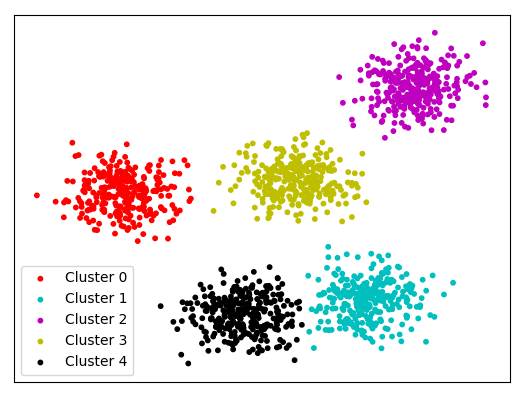
\includegraphics[width=0.5\linewidth]{k-means}}%
  \caption{K-Means algorithm applied to geolocations to reduce gps and human positioning error.}
  \label{fig:k-means-clustering}
\end{figure}

The pre-requisites for the application development have been gathered from meeting with the FitoAgro group and a shared Google Drive folder with the protocols for biological sampling as described in \ref{sec:problem_pests}.

\section{Development plan}

This section serves as description of the major tasks illustrated in figure \ref{fig:gantt}.

\begin{figure}[htbp]
  \centering
  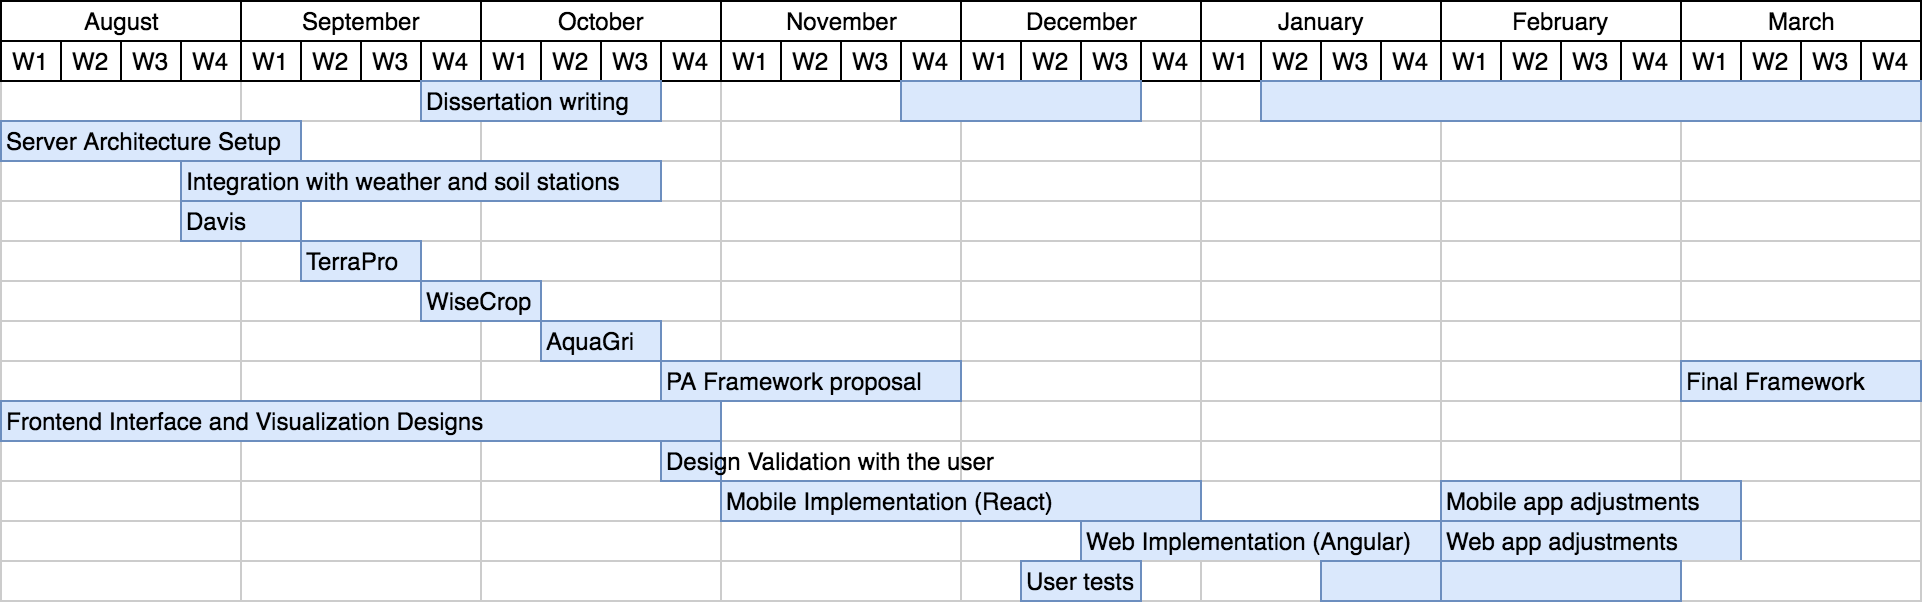
\includegraphics[width=1.5\linewidth, angle=90]{gantt}
  \caption{Gantt chart illustrating the planning of the work proposed by this dissertation.}
  \label{fig:gantt}
\end{figure}

Server Architecture Setup - Technological stack decisions, version control, Trello board for coordination and development setup with proper tools for modern web/mobile development.

Integration with weather and soil stations - Common brands for weather and soil stations amongst the FitoAgro partners are: Davis, TerraPro, WiseCrop and AquaGri. Integration with their APIs or scrapping their content should take, two weeks per brand. 

Frontend Interface and Visualization Designs - The development of the visualization proposal showcased in \ref{fig:vis_pers_highlevel} \ref{fig:vis_2d_highlevel} will be resumed during the station integrations. This work will consider interactions, attribute based maps, screen real estate, layered organization and user experience patterns.

Mobile Application Implementation in React - Implementation of the data collection application core components: a georeferenced enemy tracking registering interface with offline usage, media management attached to biological observations and rich visualizations if the task on interface and visualization designs deems appropriate for mobile usage.

Web Application Implementation in Angular - Implementation of the extended version of the interface with full visualization screens: risk maps, soil maps, weather and pest distribution maps. These visualizations may suffer changes if requested by the FitoAgro project group or from the Agronomy experts from ISA.

Proper user testing time is allocated in the Gantt chart (figure \ref{fig:gantt}) during the final phases of mobile and web interfaces. These will consist of predefined user stories for the end-user to execute \emph{in situ}. Rates of correct execution and time taken to perform each action will be logged in order to access the user-experience of the framework developed.
